\documentclass[tikz,border=3pt]{standalone}
\usepackage[T1]{fontenc}
\usepackage{newtxtext,newtxmath}
\usetikzlibrary{arrows.meta,calc}
\definecolor{ink}{HTML}{23343F}
\definecolor{blue}{HTML}{2276A0}
\definecolor{orange}{HTML}{C46B2C}
\definecolor{teal}{HTML}{087F78}
\definecolor{gray}{HTML}{4C5D67}
\definecolor{rule}{HTML}{D6DFE3}
\begin{document}
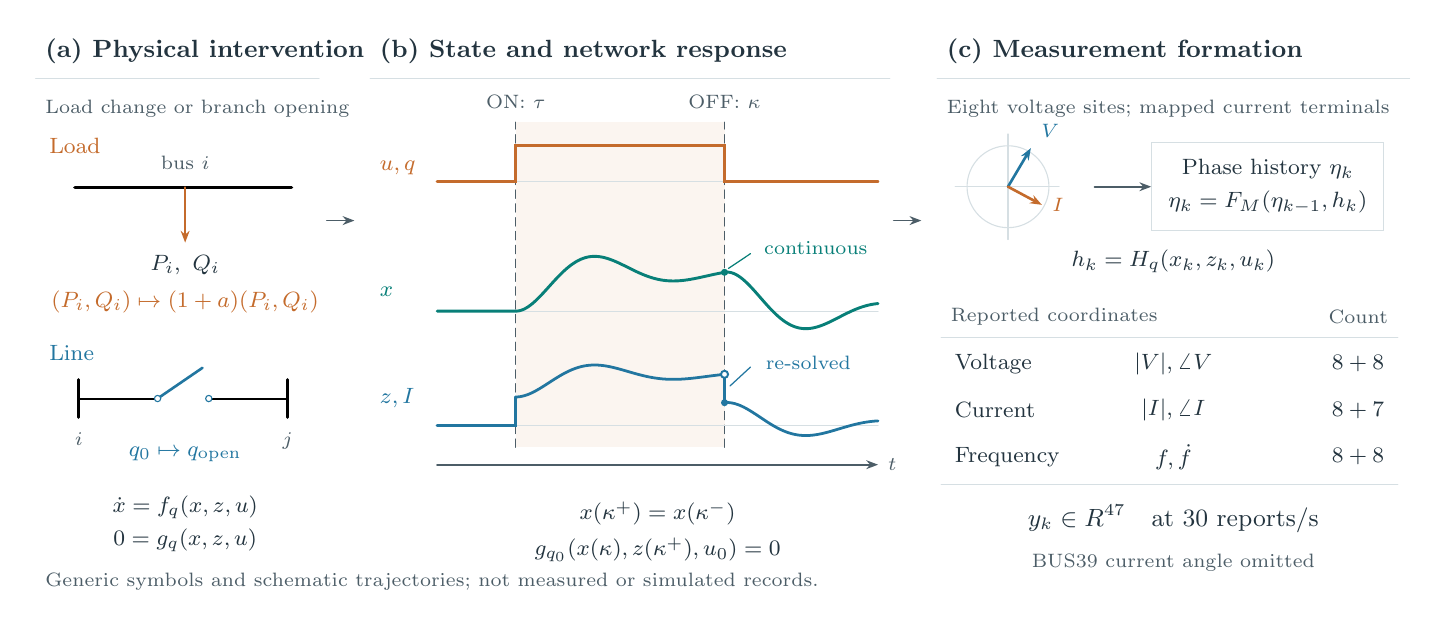
\begin{tikzpicture}[font=\fontsize{8.3}{10}\selectfont,text=ink,
 >={Stealth[length=1.5mm]},line cap=round,
 head/.style={anchor=west,font=\bfseries\fontsize{9.2}{11}\selectfont},
 note/.style={font=\fontsize{7.5}{9}\selectfont,text=gray},
 guide/.style={draw=rule,line width=.4pt},
 flow/.style={->,draw=gray,line width=.65pt}]
\path[use as bounding box] (0,0) rectangle (17.7,7.15);
\node[head] at (.1,6.85) {(a) Physical intervention};
\node[head] at (4.35,6.85) {(b) State and network response};
\node[head] at (11.55,6.85) {(c) Measurement formation};
\draw[guide] (.1,6.5)--(3.7,6.5) (4.35,6.5)--(10.95,6.5) (11.55,6.5)--(17.55,6.5);
\node[note,anchor=west] at (.1,6.12) {Load change or branch opening};
% Conventional symbols use arbitrary i,j labels, not an invented IEEE topology.
\node[text=orange,anchor=west] at (.15,5.65) {Load};
\draw[line width=1.3pt] (.6,5.12)--(3.35,5.12);
\node[note,above] at (2,5.22) {bus $i$};
\draw[orange,->,line width=.95pt] (2,5.12)--(2,4.42);
\node at (2,4.14) {$P_i,\ Q_i$};
\node[text=orange] at (2,3.67) {$(P_i,Q_i)\mapsto(1+a)(P_i,Q_i)$};
\node[text=blue,anchor=west] at (.15,3.02) {Line};
\draw[line width=1.1pt] (.65,2.2)--(.65,2.68) (3.3,2.2)--(3.3,2.68);
\draw[line width=.7pt] (.65,2.44)--(1.65,2.44) (2.3,2.44)--(3.3,2.44);
\draw[blue,line width=.95pt] (1.65,2.44)--(2.22,2.83);
\draw[blue,fill=white] (1.65,2.44) circle (.04) (2.3,2.44) circle (.04);
\node[note,below] at (.65,2.13) {$i$};\node[note,below] at (3.3,2.13) {$j$};
\node[text=blue] at (2,1.73) {$q_0\mapsto q_{\mathrm{open}}$};
\node[align=center] at (2,.85) {$\dot x=f_q(x,z,u)$\\[2pt]$0=g_q(x,z,u)$};
\draw[flow] (3.8,4.7)--(4.15,4.7);
% Shared event clock; response is an illustrative damped second-order pulse.
\def\ta{6.2}\def\ka{8.85}
\fill[orange!7] (\ta,1.82) rectangle (\ka,5.95);
\foreach \xx/\lab in {\ta/{ON: $\tau$},\ka/{OFF: $\kappa$}} {
 \draw[gray,densely dashed,line width=.45pt] (\xx,1.82)--(\xx,5.95);
 \node[note,above] at (\xx,6) {\lab};
}
\node[text=orange,anchor=west] at (4.35,5.37) {$u,q$};
\node[text=teal,anchor=west] at (4.35,3.8) {$x$};
\node[text=blue,anchor=west] at (4.35,2.45) {$z,I$};
\foreach \yy in {5.2,3.55,2.1} {\draw[guide] (5.2,\yy)--(10.8,\yy);}
\draw[orange,line width=1pt] (5.2,5.2)--(\ta,5.2)--(\ta,5.65)--(\ka,5.65)--(\ka,5.2)--(10.8,5.2);
\pgfmathdeclarefunction{resp}{1}{\pgfmathparse{#1<0 ? 0 : 1-exp(-.8*#1)*(cos(180*#1)+.8/pi*sin(180*#1))}}
\draw[teal,line width=1.05pt] plot[domain=5.2:10.8,samples=200] (\x,{3.55+.48*(resp(\x-6.2)-resp(\x-8.85))});
\fill[teal] (\ka,{3.55+.48*resp(2.65)}) circle (.045);
\node[note,text=teal,anchor=west] at (9.23,4.35) {continuous};
\draw[teal,line width=.45pt] (9.18,4.28)--(8.9,{3.6+.48*resp(2.65)});
\draw[blue,line width=1pt] (5.2,2.1)--(\ta,2.1)--(\ta,2.46);
\draw[blue,line width=1pt] plot[domain=6.2:8.85,samples=100] (\x,{2.46+.28*resp(\x-6.2)});
\draw[blue,line width=1pt] (\ka,{2.46+.28*resp(2.65)})--(\ka,{2.1+.28*resp(2.65)});
\draw[blue,line width=1pt] plot[domain=8.85:10.8,samples=80] (\x,{2.1+.28*(resp(\x-6.2)-resp(\x-8.85))});
\draw[blue,fill=white,line width=.7pt] (\ka,{2.46+.28*resp(2.65)}) circle (.045);
\fill[blue] (\ka,{2.1+.28*resp(2.65)}) circle (.045);
\node[note,text=blue,anchor=west] at (9.25,2.9) {re-solved};
\draw[blue,line width=.45pt] (9.18,2.84)--(8.92,2.6);
\draw[flow] (5.2,1.6)--(10.8,1.6) node[right,note] {$t$};
\node at (8,.98) {$x(\kappa^+)=x(\kappa^-)$};
\node at (8,.52) {$g_{q_0}(x(\kappa),z(\kappa^+),u_0)=0$};
\draw[flow] (11.0,4.7)--(11.35,4.7);
% A phasor glyph encodes magnitude and phase; f and ROCOF use phase memory.
\node[note,anchor=west] at (11.55,6.12) {Eight voltage sites; mapped current terminals};
\draw[guide] (12.45,5.13) circle (.52);
\draw[guide] (11.78,5.13)--(13.1,5.13) (12.45,4.46)--(12.45,5.8);
\draw[blue,->,line width=.95pt] (12.45,5.13)--(12.74,5.62) node[above right,font=\fontsize{7}{9}\selectfont] {$V$};
\draw[orange,->,line width=.95pt] (12.45,5.13)--(12.88,4.9) node[right,font=\fontsize{7}{9}\selectfont] {$I$};
\node[draw=rule,inner sep=6pt,align=center] (memory) at (15.75,5.13) {Phase history $\eta_k$\\[2pt]$\eta_k=F_M(\eta_{k-1},h_k)$};
\draw[flow] (13.55,5.13)--(memory.west);
\node at (14.55,4.18) {$h_k=H_q(x_k,z_k,u_k)$};
\node[note,anchor=west] at (11.6,3.48) {Reported coordinates};
\node[note,anchor=east] at (17.4,3.48) {Count};
\draw[guide] (11.6,3.22)--(17.4,3.22);
\foreach \yy/\name/\math/\count in {2.88/Voltage/{$|V|,\angle V$}/{$8+8$},2.29/Current/{$|I|,\angle I$}/{$8+7$},1.7/Frequency/{$f,\dot f$}/{$8+8$}} {
\node[anchor=west] at (11.65,\yy) {\name};
\node at (14.55,\yy) {\math};
\node[anchor=east] at (17.35,\yy) {\count};
}
\draw[guide] (11.6,1.35)--(17.4,1.35);
\node[font=\fontsize{9}{11}\selectfont] at (14.55,.91) {$y_k\in\mathbb R^{47}$\quad at 30 reports/s};
\node[note] at (14.55,.35) {BUS39 current angle omitted};
\node[note,anchor=west] at (.1,.12) {Generic symbols and schematic trajectories; not measured or simulated records.};
\end{tikzpicture}
\end{document}
